\chapter{Development Process}

\textcolor{orange}{NOE TEKST}

\section{Code Repositories}

% Github Organization and repos
All code and project-related resources are stored on GitHub under a dedicated organization\footnote{\url{https://github.com/skogkursbachelor}}. Each component of the system, as well as supporting documentation, is maintained in its own repository. This modular structure facilitates collaboration and version control throughout the development process.

An overview of the repositories and their respective purposes is shown in \hyperref[tab:github_repositories]{Table \ref*{tab:github_repositories}}.

\begin{table}[h]
    \centering
    \begin{tabular}{l|l}
        \hline
        \textbf{Repository} & \textbf{Description} \\
        \hline
        server & The code for the backend server. \\
        website & The code for the website. \\
        \hline
        meetingminutes & A backup of all meeting minutes. \\
        diagrams & A backup of all diagrams. \\
        thesis & A backup version of the thesis. \\
        projectplan & A backup version of the project plan. \\
        \hline
    \end{tabular}
    \caption{Overview of all GitHub repositories\footnotemark}
    \label{tab:github_repositories}
\end{table}
\footnotetext{\url{https://github.com/orgs/skogkursbachelor/repositories}}

\section{Time Tracking}

All project work was tracked using the self-hosted time tracking service Traggo\footnote{\url{https://traggo.net/}}. Traggo tracks work by tags making it easy to get an overview of time spent on different tasks.

\begin{table}[h]
    \centering
    \begin{tabular}{c|c|c|c}
        \hline
        \textbf{Month} & \textbf{Bjørnsen} & \textbf{Houmb} & \textbf{Total} \\
        \hline
        January  & 61h 39m  & 62h 58m  & 124h 37m \\
        February & 80h 6m   & 79h 17m  & 159h 24m \\
        March    & 88h 4m   & 88h 20m  & 176h 24m \\
        April    & 35h 36m  & 31h 18m  & 66h 54m \\
        May      &        &        &        \\
        \hline
        Total & & & \\
        \hline
    \end{tabular}
    \caption{Tracked time by month and group member}
    \label{tab:tracked_time_by_month_member}
\end{table}

% Skriv mer om time fordeling, f.eks. hvorfor mer timer i mars enn januar etc.
\hyperref[tab:tracked_time_by_month_member]{Table \ref*{tab:tracked_time_by_month_member}} shows the total time of work for each month by the two members.

% KANSKJE IKKE TA SKJERMBILDE, LAG HELLER CHART MED LATEX f.eks. (pfg-pie).
\begin{figure}[h]
    \centering
    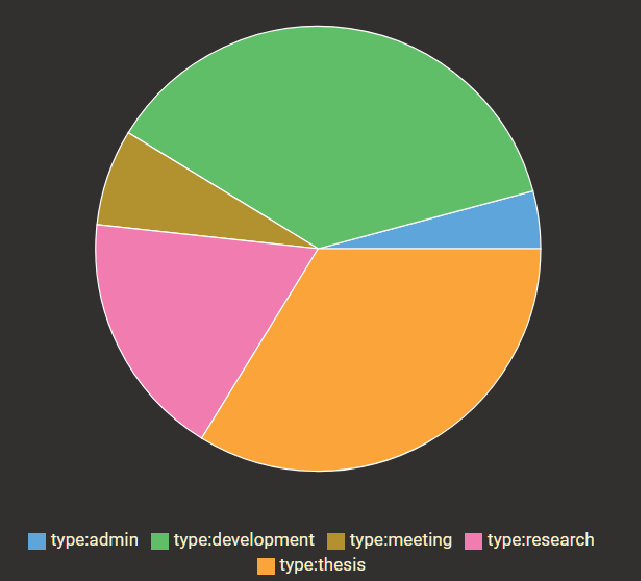
\includegraphics[width=0.5\linewidth]{figures/time_tracking_by_type.pdf}
    \caption{Pie chart of time spent in total per work type}
    \label{fig:time_tracking_by_type}
\end{figure}

% SKRIV OM TIDSFORDELING FOR DE FORSKJELLIGE OPPGAVENE (THESIS, DEV, osv.)

To provide an overview of the project timeline, a Gantt chart was created, highlighting the different sprints and key milestones. A more detailed table of all dates referenced in the Gantt chart can be found in \hyperref[appendix:project_plan]{Appendix \ref*{appendix:project_plan}}.

\section{Gantt Diagram}

\textcolor{orange}{NOE TEKST}
\begin{figure}[h]
    \centering
        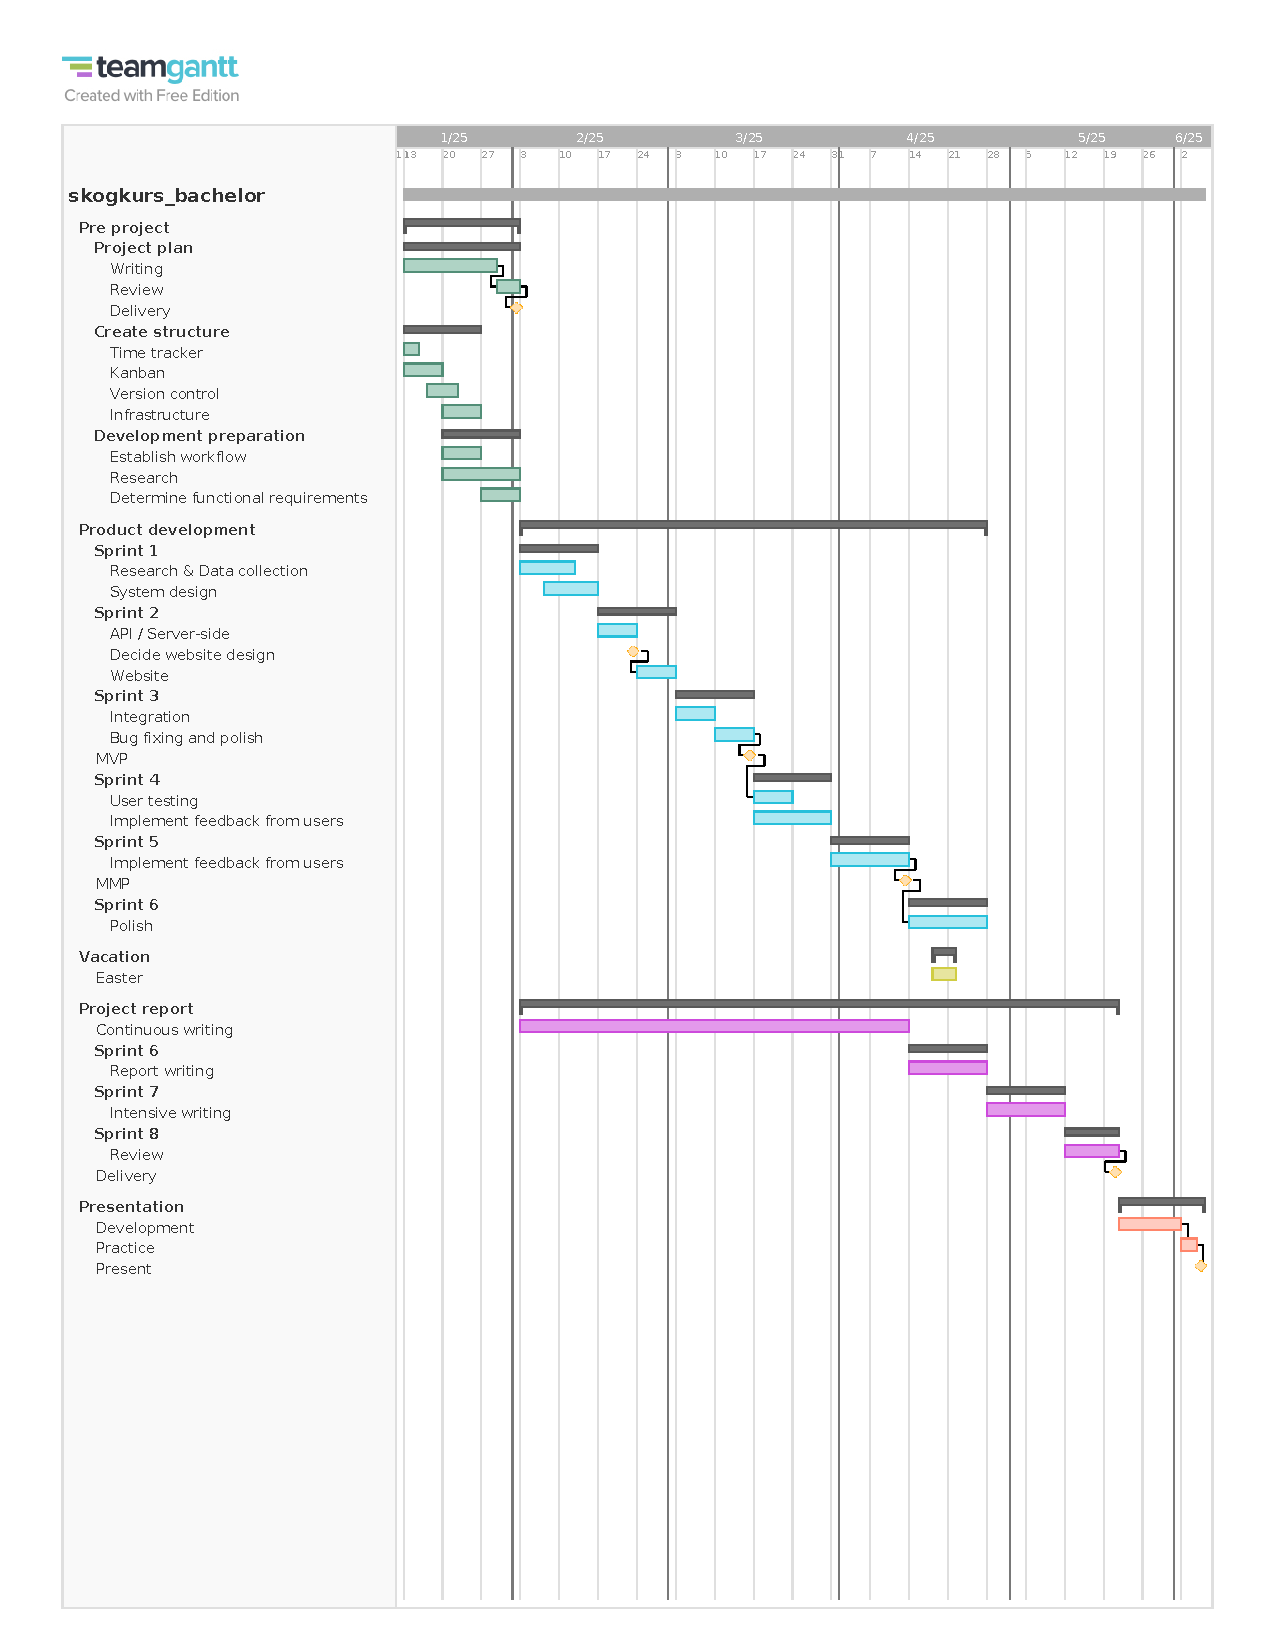
\includegraphics[width=1.0\linewidth, trim=0 60mm 0 20mm, clip]{figures/skogkurs_bachelor_gantt.pdf}
    \caption{Gantt diagram of the project}
    \label{fig:gantt_diagram}
\end{figure}

\section{Software Development Lifecycle Model}

For this project, the team needed to select an appropriate Software Development Lifecycle (\acrshort{sdlc}) model. Key factors considered in this decision included the clarity and flexibility of the requirements, team size, project timeline, product delivery goals, and prior experience \cite{sdlc_model}. 
\\ \\
The requirements provided by the Product Owner are intentionally ambiguous and flexible, allowing the team to prioritize the few fixed requirements upfront while iteratively refining the flexible ones over time. The team is composed of two members with similar experience levels, enabling close collaboration and effective decision-making. With a short project timeline of four months, a structure of 2-week sprints aligns perfectly with Scrum's iterative and adaptive approach, ensuring steady progress and regular opportunities for feedback. 
\\ \\
Since our project lacks clearly defined requirements and requires ongoing collaboration with the Product Owner, Scrum was the best fit for our team and project. Traditional methodologies like Waterfall were not suitable, as they rely on fixed requirements and a linear development process, which would limit our flexibility. Extreme Programming (XP), while valuable for high-collaboration environments with strict engineering practices like pair programming and test-driven development, was not fully suitable as our project does not emphasize these practices to the same extent \cite{extreme_programming}. Similarly, Lean development focuses on minimizing waste and maximizing efficiency but is less structured in terms of iterative planning, which we need to manage evolving requirements effectively \cite{lean_programming}. By adopting Scrum, we can iteratively refine requirements and adapt to changes throughout development \cite{sdlc_model}. To implement Scrum effectively, several key practices will be integrated into our workflow \cite{scrum_guide}.

\begin{itemize}
    \item \textbf{Sprint Meetings:} The project will be divided into 2-week sprints. At the start of each sprint, sprint meetings will include sprint planning, reviews, and retrospectives. During the planning phase, the team will select tasks from the product backlog to form the sprint backlog for the upcoming sprint. The review phase will focus on assessing progress and determining whether adjustments to the product backlog are needed. The retrospective phase will identify areas for improvement in the Scrum process itself.
    \item \textbf{Daily Scrum Meetings:} Short daily meetings will be conducted to discuss the progress of ongoing tasks, identify potential obstacles, and ensure alignment between team members.
    \item \textbf{Scrum Master:} Given that the team consists of only two members, we have decided to share the role of Scrum Master. Both members are responsible for ensuring adherence to the Scrum framework and continuously working to improve team efficiency. This collaborative approach allows us to maintain flexibility while upholding Scrum principles throughout the project.
    \item \textbf{Kanban:} To complement Scrum and further enhance workflow visibility, the team will utilize a Kanban board to track and manage tasks on GitHub. The Kanban board will consist of columns representing different stages of the workflow, such as Product Backlog, Sprint Backlog, In Progress, In Review, Done, and Discarded.
\end{itemize}

\section{Sprints}

\textcolor{orange}{PUTTE HVERTFALL SPRINTREFERATENE I VEDLEGG, MEN KAN SKRIVE NOE OM SPRINTS}
% Kanskje peke til vedlegg?
% Sammenlign med det som står over, ta med sprint planning, reviews og retrospective

\subsection{Sprint 1: 03.02.2025 - 14.02.2025}
\begin{comment}
- Fyll ut Product Backlog
- Undersøke forskjellige datakilder for kart- og geodata
    - Senorge (https://api.nve.no/doc/gridtimeseries-data-gts/)
	- Geonorge (løsmasser, skogsbilveg)
	- NGU
	- NIBIO 
- System Design (?)
    - Sequence Diagram
	- Use Case Diagram
	- Activity Diagram
	- Component Diagram
\end{comment}
The primary objectives of the first sprint were to populate the product backlog for the entire project and to research potential sources of map and weather data. Data sources that were already under consideration or recommended by the product owner included:
\begin{itemize} 
    \item Senorge
    \item Geonorge
    \item NGU
    \item NIBIO
\end{itemize}

From these source the map layers for superficial deposits, frost depth, soil moisture, and forestry roads were selected using a WMS.

Additionally, the sprint included the development of the initial system diagrams. 

With the primary tasks completed, the remaining time in the sprint was used to begin developing the website. This included familiarizing with the OpenLayers library and testing the integration of the selected map layers.

\subsection{Sprint 2: 17.02.2025 - 28.02.2025}
\begin{comment}
## Hvordan gikk forrige sprint
- Fikk gjort alt i sprint back-loggen
- Bestemte oss for å begynne å utvikle nettsiden for å få testet ut de forskjellige kartlagene / geodataene
## Hva gjøre i løpet av neste sprint
- Implementere datakildene inn i nettsiden:
	- Markfuktighet
	- Grunnvann
	- Teledyp
	- Skogsbilveger
\end{comment}
This sprint was mainly focused on implementing the website and the required features. The integration of each map layer was finished and an initial version of the website was shown to the product owner.  

\subsection{Sprint 3: 03.03.2025 - 14.03.2025}
\begin{comment}
## Hvordan gikk forrige sprint
- Fikk laget ferdig en versjon vi var fornøyd med å vise frem til produkteier
- Fikk implementert disse datakildene:
	- Løsmasser
	- Teledyp
	- Markfuktighet
	- Jordfuktighet (historisk)
	- Skogsbilveger
## Hva gjøre i løpet av neste sprint
- Få prognose av jordfuktighet (open-meteo, hvis ingen bedre løsning)
- Lage en måte for å konvertere open-meteo data til geojson (eller andre format som passer til openlayers)
- Lage klassifiseringssystemet av skogsbilveger (rød, gul, grønn)
\end{comment}
In this sprint the objective was to start creating the classification system for forestry roads. 

\subsection{Sprint 4: 17.03.2025 - 28.03.2025}
\begin{comment}
## Hvordan gikk forrige sprint
- Å implementere open-meteo som kilde ble nedprioritert i forhold til klassifiseringen av skogsbilveg.
- Fikk begynt på skogsbilveg klassifiseringen, men på grunn av eksamen i et annet fag, ble det ikke ferdig.
- Fant en annen kilde hos MET for jordtemperatur og -fukt, m.m., men kun 3 dagers prognose.
- Gikk ned fra 40-45 timer på 2 uker til ca 20 timer som viser at fokuset ikke var fullt på bacheloroppgaven.
- Fikk satt opp første utkast av strukturen til rapporten og notert ned smått på enkelte kapittel.
## Hva gjøre i løpet av neste sprint
- Fullføre klassifiseringen av skogsbilvegene og samhandlingen med andre kartlag.
- Implementere selve klassifiseringsfunksjonene i backend.
- Fortsette med rapporten.
- Den planlagte brukertesten av MVP-en (ifølge Gantt-diagrammet) blir flyttet til neste sprint.   
\end{comment}

\subsection{Sprint 5: 31.03.2025 - 11.04.2025}

\textcolor{orange}{NOE TEKST}

\subsection{Sprint 6: 14.04.2025 - 25.04.2025}

\textcolor{orange}{NOE TEKST}

\subsection{Sprint 7: 28.04.2025 - 09.05.2025}

\textcolor{orange}{NOE TEKST}

\subsection{Sprint 8: 12.05.2025 - 20.05.2025}

\textcolor{orange}{NOE TEKST}

\section{Minimum Viable Product}

A Minimum Viable Product (MVP) is a concept that focuses on learning about customers with minimal effort. An MVP is an early version of a product designed to test whether customers will use or buy it, often taking the form of a simple prototype, landing page, or manually operated service. The key benefit of an MVP is that it allows teams to validate ideas early, minimizing wasted effort on products that may not succeed \cite{agile_alliance_mvp}. 

During the development of the website, we conducted user testing to gain insights into how the target audience (transport managers) would interact with the product and identify any missing features or necessary improvements. For the MVP, we prioritized implementing the core functionalities we believed users would need, as illustrated in the use case diagram in \hyperref[fig:use_case_diagram]{Figure \ref*{fig:use_case_diagram}}. Further details about the user testing process and findings are discussed in a later chapter.

\section{Minimum Marketable Product}

A Minimum Marketable Product (MMP) is the next step after an MVP in product development. While an MVP focuses on testing assumptions and user preferences, an MMP includes essential features that meet customer needs, provide a good user experience, and generate business value. It is designed to launch quickly with must-have functionality, avoiding unnecessary features that add complexity without value. The MMP approach involves refining the product to only what is essential for success. Typically, teams first develop MVPs to gather insights, then use these findings to build an MMP ready for general release. In agile development, combining MVPs and MMPs helps streamline product evolution while minimizing risk and unnecessary work \cite{wanner_mmp}. 

After conducting the user testing we used the feedback given to improve the product and ultimately reaching an MMP. 
